\subsection{Question 8}

  \subsubsection{Image \texttt{triangle128}}

    \begin{figure}[H]
      \centering
      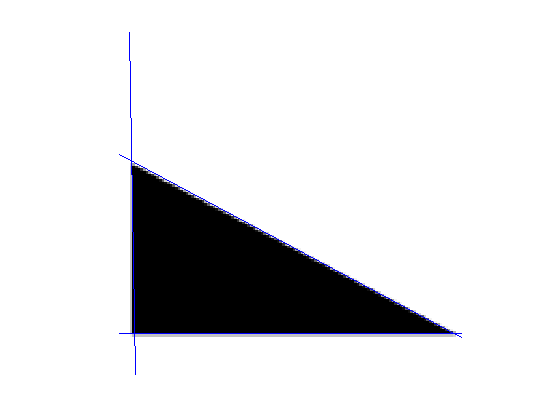
\includegraphics[scale=0.8]{./images/Q8/triangle128/1.png}
      \caption{The $3$ strongest line segments detected in image
        \texttt{triangle128} overlaid on top of it. $(scale, threshold) = (4,4)$.}
      \label{fig:Q8_triangle128_1}
    \end{figure}

    \begin{figure}[H]
      \centering
      
\includegraphics[scale=0.8]{./images/Q8/triangle128/2.png}
      \caption{The above $3$ lines in Hough space.}
      \label{fig:Q8_triangle128_2}
    \end{figure}

    \begin{figure}[H]
      \centering
      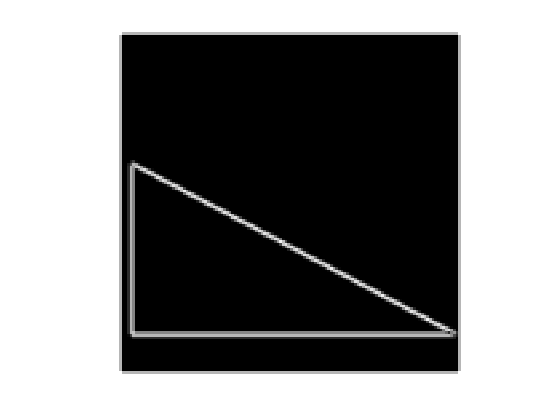
\includegraphics[scale=0.8]{./images/Q8/triangle128/3.png}
      \caption{The gradient of image \text{triangle128}.}
      \label{fig:Q8_triangle128_3}
    \end{figure}

    \begin{figure}[H]
      \centering
      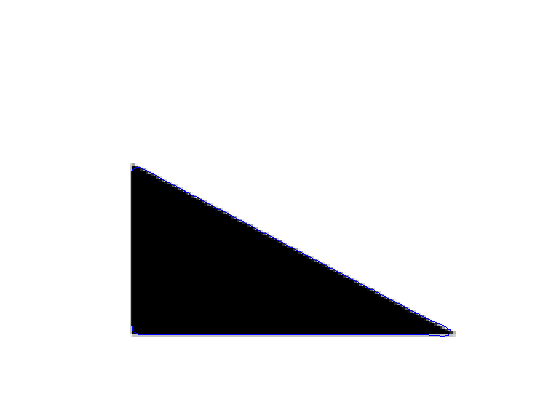
\includegraphics[scale=0.8]{./images/Q8/triangle128/4.png}
      \caption{The edges detected in image \text{triangle128} for
        $(scale, threshold) = (4,4)$.}
      \label{fig:Q8_triangle128_4}
    \end{figure}


  \subsubsection{Image \texttt{houghtest256}}

    \begin{figure}[H]
      \centering
      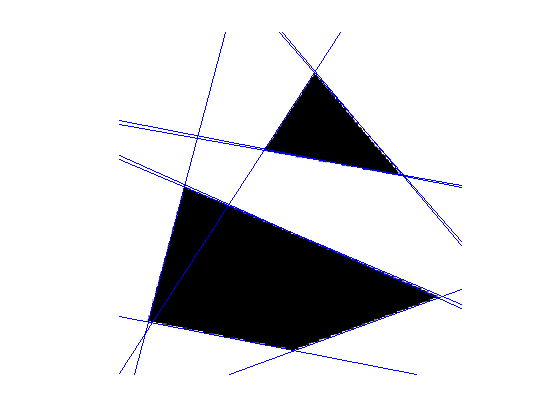
\includegraphics[scale=0.8]{./images/Q8/houghtest256/1.png}
      \caption{The $10$ strongest line segments detected in image
        \texttt{houghtest256} overlaid on top of it. $(scale, threshold) = (4,4)$.}
      \label{fig:Q8_houghtest256}
    \end{figure}

    \begin{figure}[H]
      \centering
      
\includegraphics[scale=0.8]{./images/Q8/houghtest256/2.png}
      \caption{The above $10$ lines in Hough space.}
      \label{fig:Q8_houghtest256}
    \end{figure}

    \begin{figure}[H]
      \centering
      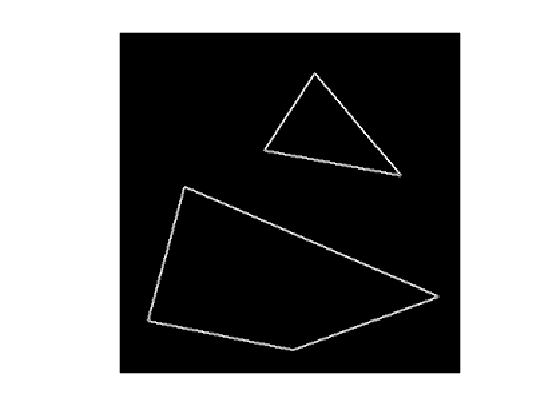
\includegraphics[scale=0.8]{./images/Q8/houghtest256/3.png}
      \caption{The gradient of image \text{houghtest256}.}
      \label{fig:Q8_houghtest256_3}
    \end{figure}

    \begin{figure}[H]
      \centering
      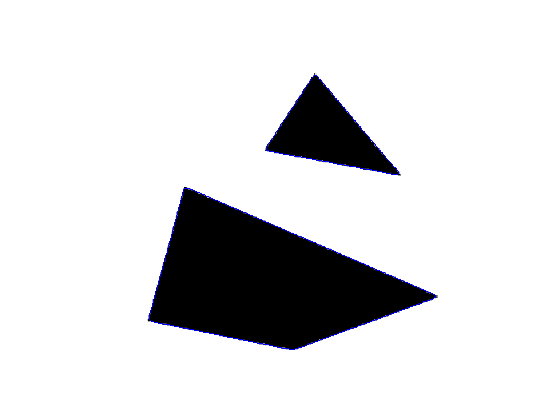
\includegraphics[scale=0.8]{./images/Q8/houghtest256/4.png}
      \caption{The edges detected in image \text{houghtest256} for
        $(scale, threshold) = (4,4)$.}
      \label{fig:Q8_houghtest256_4}
    \end{figure}


  \subsubsection{Image \texttt{few256}}

    \begin{figure}[H]
      \centering
      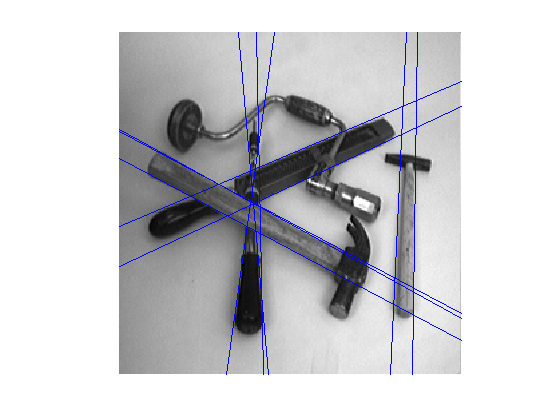
\includegraphics[scale=0.8]{./images/Q8/few256/1.png}
      \caption{The $10$ strongest line segments detected in image
        \texttt{few256} overlaid on top of it. $(scale, threshold) = (4,4)$.}
      \label{fig:Q8_few256_1}
    \end{figure}

    \begin{figure}[H]
      \centering
      
\includegraphics[scale=0.8]{./images/Q8/few256/2.png}
      \caption{The above $10$ lines in Hough space.}
      \label{fig:Q8_few256_2}
    \end{figure}

    \begin{figure}[H]
      \centering
      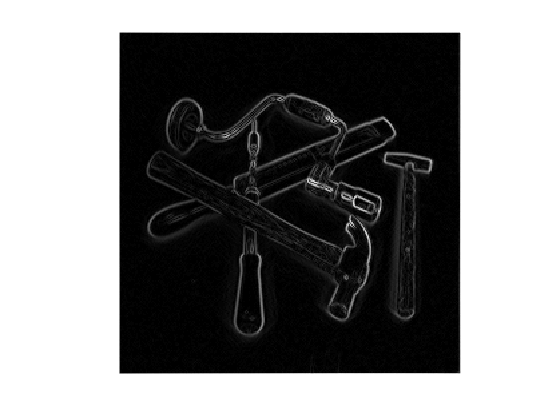
\includegraphics[scale=0.8]{./images/Q8/few256/3.png}
      \caption{The gradient of image \text{few256}.}
      \label{fig:Q8_few256_3}
    \end{figure}

    \begin{figure}[H]
      \centering
      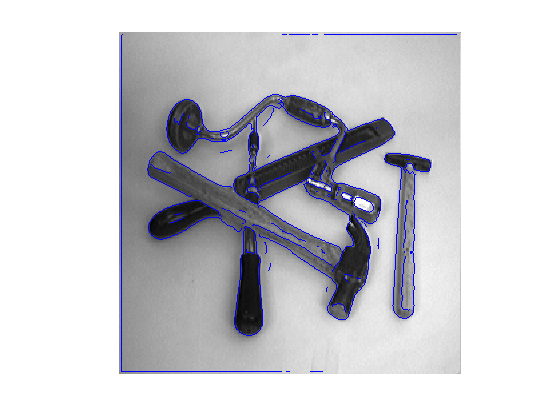
\includegraphics[scale=0.8]{./images/Q8/few256/4.png}
      \caption{The edges detected in image \text{few256} for
        $(scale, threshold) = (4,4)$.}
      \label{fig:Q8_few256_4}
    \end{figure}


  \subsubsection{Image \texttt{phonecalc256}}

    \begin{figure}[H]
      \centering
      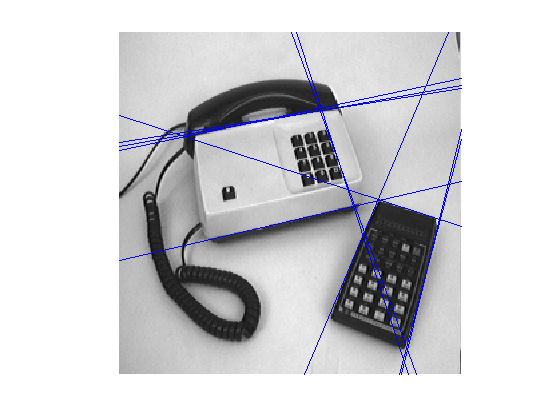
\includegraphics[scale=0.8]{./images/Q8/phonecalc256/1.png}
      \caption{The $10$ strongest line segments detected in image
        \texttt{phonecalc256} overlaid on top of it. $(scale, threshold) = (4,4)$.}
      \label{fig:Q8_phonecalc256_1}
    \end{figure}

    \begin{figure}[H]
      \centering
      
\includegraphics[scale=0.8]{./images/Q8/phonecalc256/2.png}
      \caption{The above $10$ lines in Hough space.}
      \label{fig:Q8_phonecalc256_2}
    \end{figure}

    \begin{figure}[H]
      \centering
      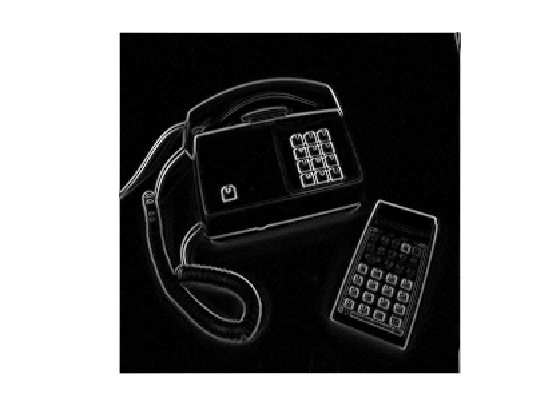
\includegraphics[scale=0.8]{./images/Q8/phonecalc256/3.png}
      \caption{The gradient of image \text{phonecalc256}.}
      \label{fig:Q8_phonecalc256_3}
    \end{figure}

    \begin{figure}[H]
      \centering
      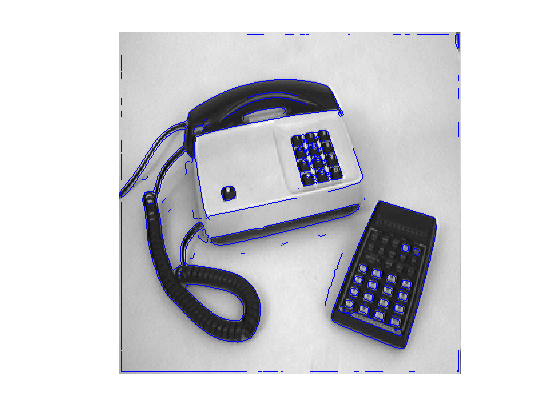
\includegraphics[scale=0.8]{./images/Q8/phonecalc256/4.png}
      \caption{The edges detected in image \text{phonecalc256} for
        $(scale, threshold) = (4,4)$.}
      \label{fig:Q8_phonecalc256_4}
    \end{figure}


  \subsubsection{Image \texttt{godthem256}}

    \begin{figure}[H]
      \centering
      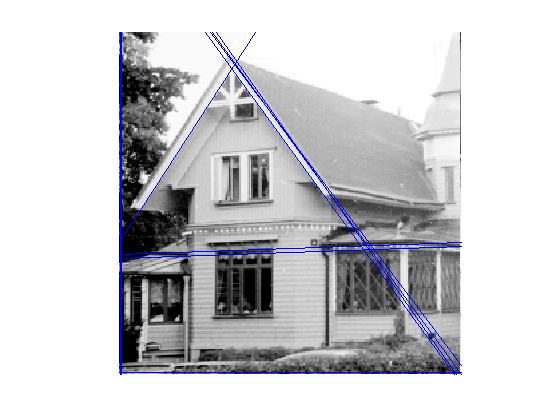
\includegraphics[scale=0.8]{./images/Q8/godthem256/1.png}
      \caption{The $10$ strongest line segments detected in image
        \texttt{godthem256} overlaid on top of it. $(scale, threshold) = (4,4)$.}
      \label{fig:Q8_godthem256_1}
    \end{figure}

    \begin{figure}[H]
      \centering
      
\includegraphics[scale=0.8]{./images/Q8/godthem256/2.png}
      \caption{The above $10$ lines in Hough space.}
      \label{fig:Q8_godthem256_2}
    \end{figure}

    \begin{figure}[H]
      \centering
      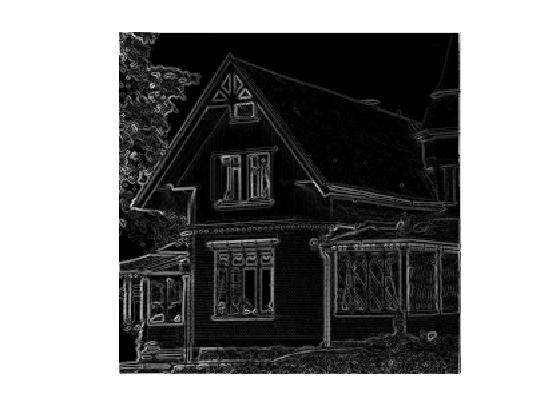
\includegraphics[scale=0.8]{./images/Q8/godthem256/3.png}
      \caption{The gradient of image \text{godthem256}.}
      \label{fig:Q8_godthem256_3}
    \end{figure}

    \begin{figure}[H]
      \centering
      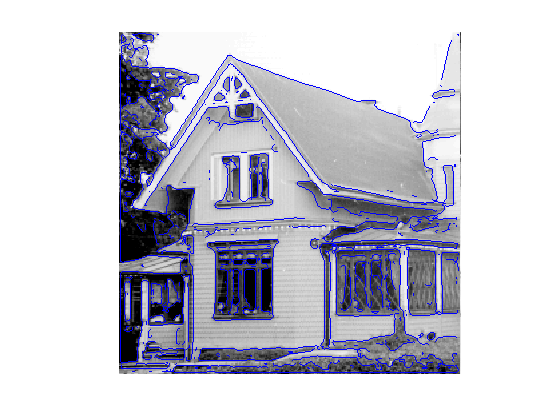
\includegraphics[scale=0.8]{./images/Q8/godthem256/4.png}
      \caption{The edges detected in image \text{godthem256} for
        $(scale, threshold) = (4,4)$.}
      \label{fig:Q8_godthem256_4}
    \end{figure}

  \subsection{Question 9}
    Since we compute $ntheta$ values for $\rho$ and there are $c$ number of
    points that lie on curves identified by the \texttt{edgecurves} function,
    the complexity is $O(ntheta \cdot c)$.

    As for the accuracy of the results, a higher resolution of the accumulator,
    that is larger values for $ntheta$ and $nrho$, increases the accuracy
    of line approximation, and lower resolution reduces it, even for small
    changes in resolution. However, the finer the detail of the accumulator
    the more local maxima are observed since the more non-zero $ntheta$ and $nrho$
    values there are in the vicinity of an otherwise single pair of
    $ntheta$ and $nrho$ values. This gives rise to multiple lines per every
    single line we wish to approximate and thus requires a higher value for
    \texttt{nlines} in order to locate more lines.


  \subsection{Question 10}
    I identify two problems here: the simple addition of $1$ in the accumulator
    and the addition of the magnitude of the gradient of that point.

    The former treats all edge points in the same manner, irrespective of the
    strength of the magnitude of the gradient in that point, which means that
    stronger edges are not represented in a fair manner, that is, they may not be
    approximated, even though it is quite obvious in the edges image that
    they should be.

    The latter, however, gives too much attention to these strong gradients
    and results in approximating them with multiple lines instead of approximating
    them once and then moving on to edges of lesser strength.

    Hence, a good choice for a monotonically increasing function is either the
    \texttt{log} or the \texttt{square root} function.


